\newpage

\section{Tilted Square}

\begin{teachingnote}
This leads to the Pythagorean Theorem.  A common misconception is to ``rotate'' the figure to become a $7\times 7$ square.  Look for multiple solution methods:  (1) counting approximately, (2) counting exactly, (2) additive and (3) subtractive approaches with triangles and squares.
\end{teachingnote}

\begin{prob}
In the diagram below, the dots are 1 centimeter apart, both vertically and horizontally.  The vertices of the square all lie exactly on such dots. Find the area of the square, \emph{without computing the length of the side of the square}.  Explain your method.  

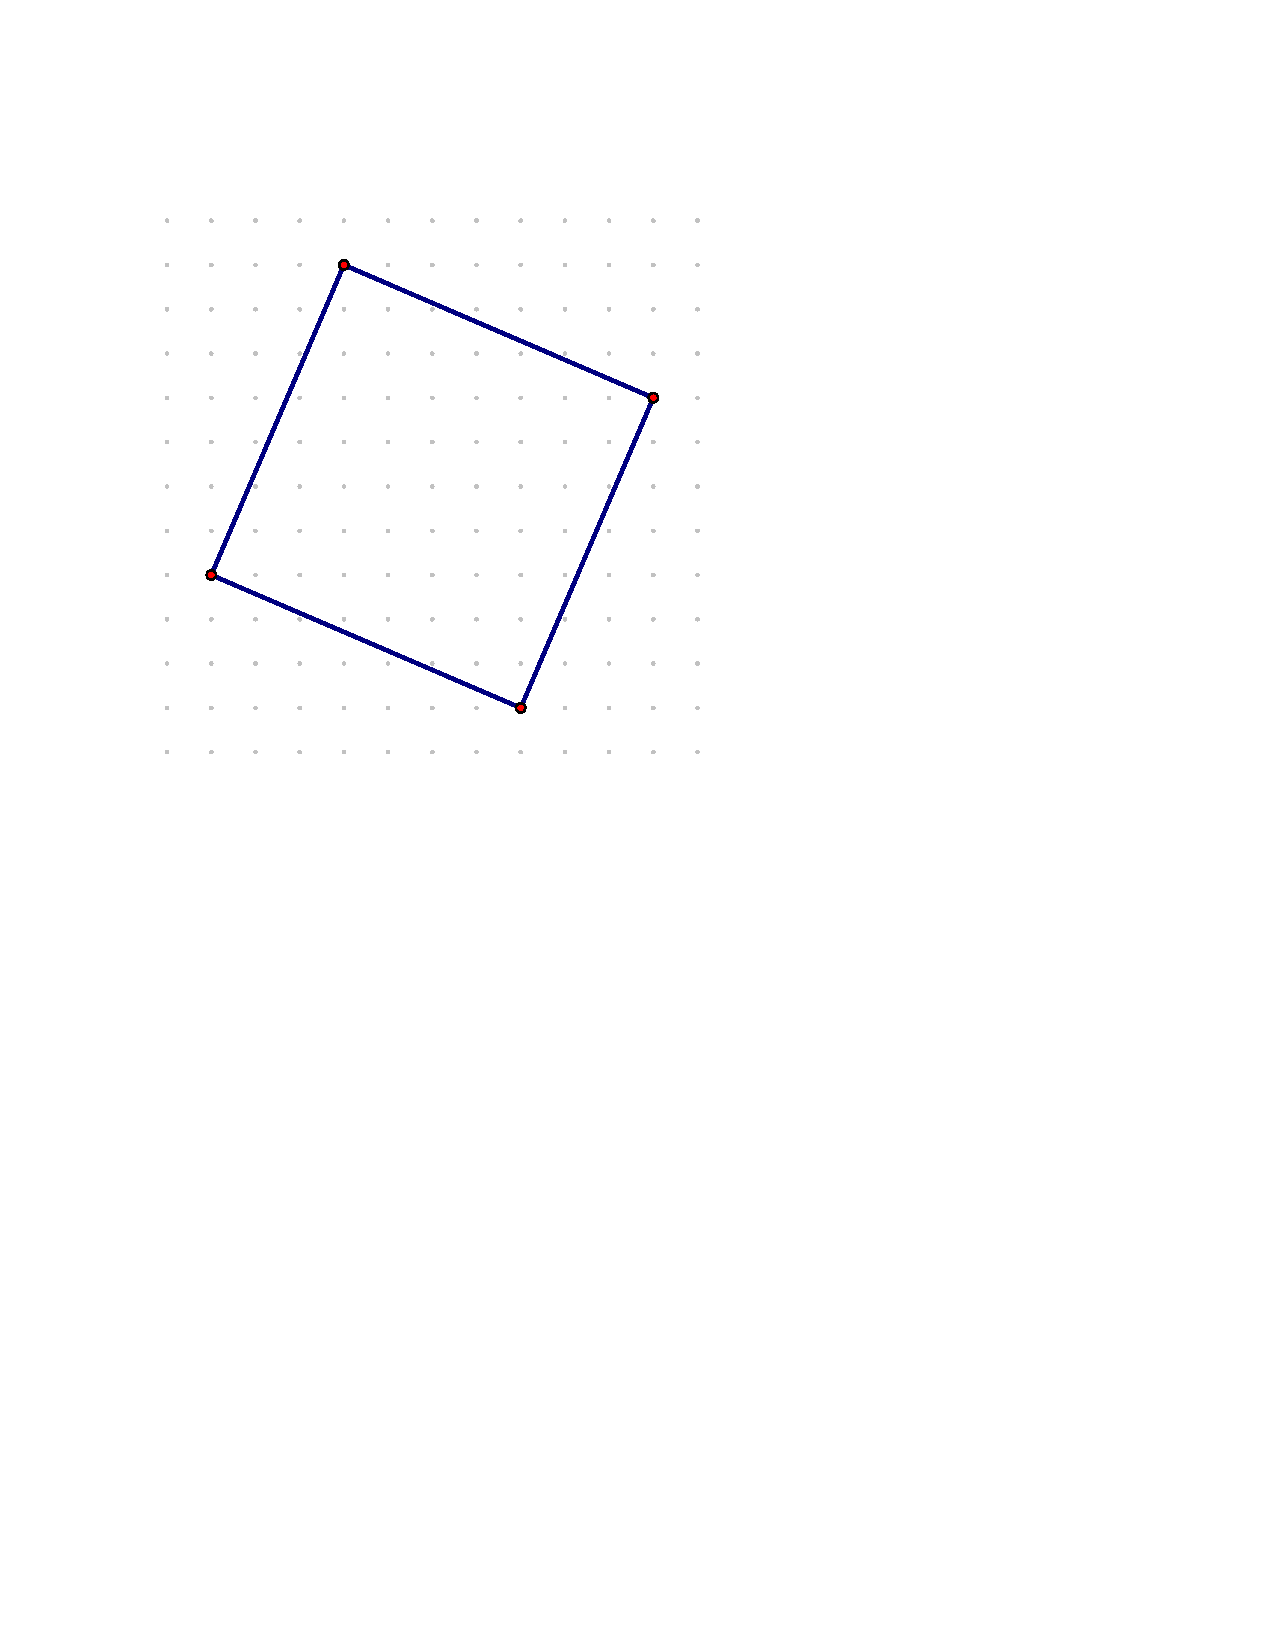
\includegraphics{../graphics/tiltedSquare}

\end{prob}
